\fancyhead{}
\fancyfoot{}


\lhead{Configurar VPN - Discadores}
\textbf{Configurar Discadores:}\\
\textbf{Connect To:} Direcci�n IP con la cual el equipo cliente se identificara en nuestra re LAN\\
\textbf{Name:} Nombre de Usuario VPN\\
\textbf{Password:} Contrase�a del Usuario VPN\\
\textbf{Profile:} Perfil de encryptacion
Escoger el men� \textbf{PPP} $\rightarrow$  \textbf{Secret}  $\rightarrow$ \textcolor{red}{\textbf{+}}\\
\begin{figure}[H]
\begin{center}
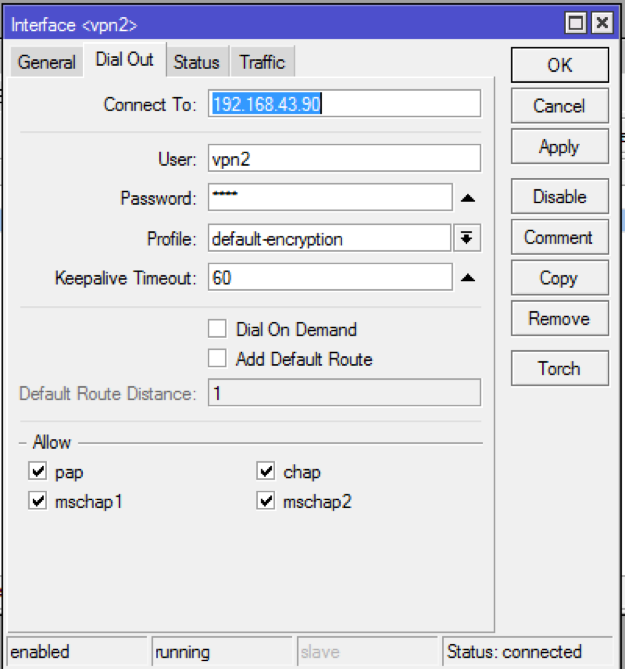
\includegraphics[scale = .5]{./figuras/figura098.png}
\caption{Datos Discador Cliente por Internet}
\label{discador-cliente-internet}
\end{center}
\end{figure}
 Escoger el men� \textbf{ppp} $\rightarrow$  \textbf{Secret}  $\rightarrow$ \textcolor{red}{\textbf{+}}\\
\begin{figure}[H]
\begin{center}
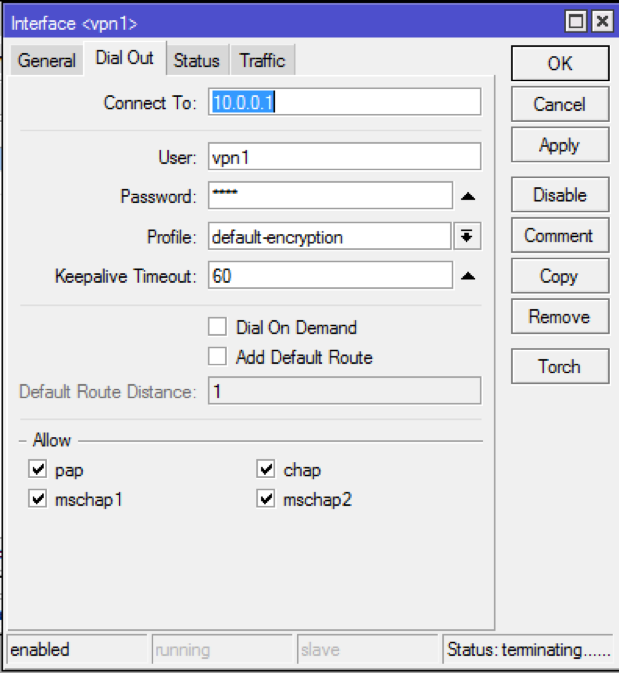
\includegraphics[scale = .5]{./figuras/figura099.png}
\caption{Datos Discador Cliente VPN por Enlace}
\label{discador-cliente-enlace}
\end{center}
\end{figure}
 Escoger el men� \textbf{IP} $\rightarrow$  \textbf{Routes} $\rightarrow$ \textcolor{red}{\textbf{+}}\\
\begin{figure}[H]
\begin{center}
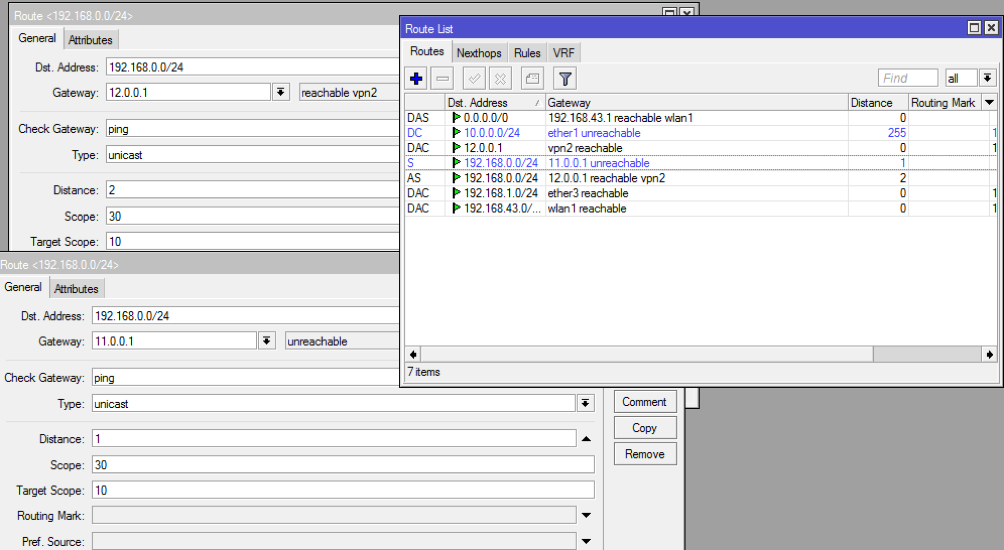
\includegraphics[scale = .5]{./figuras/figura100.png}
\caption{Configuraciones de Puertas de enlace}
\label{config-puerta-enlace}
\end{center}
\end{figure}

Escoger el men� \textbf{Inicio} $\rightarrow$  \textbf{ejecutar}  $\rightarrow$ \textbf{cmd}\\

\begin{figure}[H]
\begin{center}
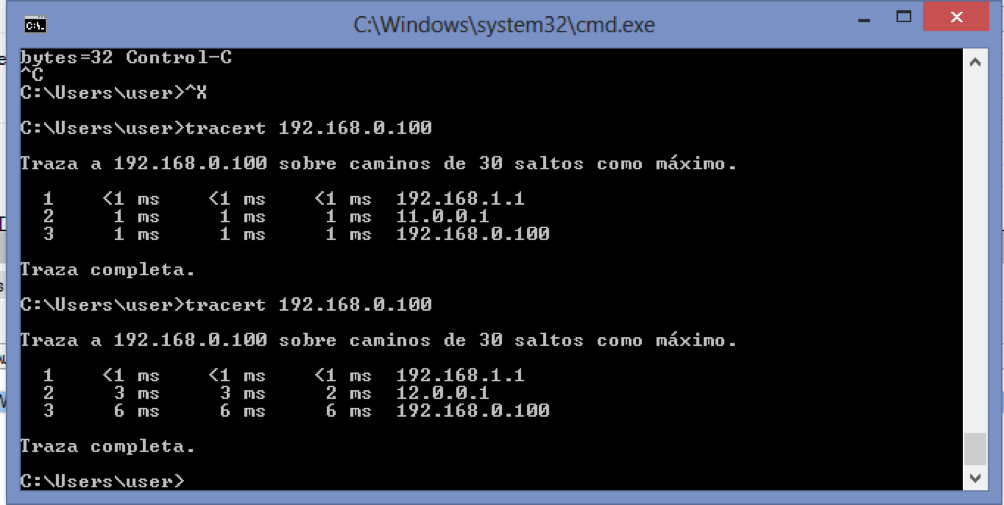
\includegraphics[scale = .5]{./figuras/figura101.png}
\caption{Prueba de \gls{traceroute} desde la maquina Sucursal 1}
\label{prueba-tracert}
\end{center}
\end{figure}